\documentclass[a4paper,12pt]{article}
\newcounter{example}[]
\newenvironment{example}[1][]{\refstepcounter{example}\par\medskip
   \noindent \textbf{Example~\theexample. #1} \rmfamily}{\medskip}
   %%%%%%%%%%%%%%%%%%%%%%%%%%%%%%%%

%%%%%%%%%%%%%%%%%%%%%%%%%%%%%%%%%%
\usepackage[utf8]{inputenc}
\usepackage[english]{babel}
\usepackage{tikz-cd}
\usepackage{amsmath,amsfonts,amssymb,amsthm}
\usepackage{mathtools}
 \usepackage{float}
\usepackage{amsthm}
\usepackage{cite}
\usepackage{datetime} % British format dates
\usepackage[cm]{fullpage}
\usepackage{url}
\usepackage{hyperref}
\usepackage{stackrel,amssymb,amsmath}
\usepackage[nottoc]{tocbibind}
\usepackage{pgfplots}
\usepackage{rotating}
\usepackage[autostyle]{csquotes}
\usepackage{natbib}
\usepackage{graphicx}
\usepackage{natbib}
\usepackage{graphicx}

\newtheorem{problem}{Problem}
\newtheorem{attempt}{Attempt}


\newtheorem{theorem}{Theorem}[section]
\newtheorem{corollary}{Corollary}[theorem]
\newtheorem{lemma}[theorem]{Lemma}
\newtheorem{proposition}[theorem]{Proposition}
\theoremstyle{definition}
\newtheorem{definition}{Definition}[section]
\theoremstyle{indented}
\newtheorem*{remark}{Remark}
\newenvironment{titlemize}[1]{%
  \paragraph{#1}
  \begin{itemize}}
  {\end{itemize}}
  
  \usepackage[T1]{fontenc}
\usepackage{imakeidx}
\makeindex[columns=3, title=Alphabetical Index, intoc]
  
  
  %%%%%%%%%%5
\newcommand{\rightarrowdbl}{\rightarrow\mathrel{\mkern-14mu}\rightarrow}

\newcommand{\xrightarrowdbl}[2][]{%
  \xrightarrow[#1]{#2}\mathrel{\mkern-14mu}\rightarrow
}
%%%%%%%%%%%%%%5

\title{Region counting with super-additive functions}
\author{Rhys Wells}
\date{\today}

\begin{document}

\maketitle
\tableofcontents

\section{Questions/ Confusions/ Tasks}

\begin{titlemize}{Question for Now}
         \item Done: Is the only way to defining $f$ is through its value i.e. giving a value for each subset? I have assumed functions are determined by their values and functions act on all subsets of the power set. (Ans: Yes it is).
         \item Done: How does the value on the higher level $\{1,2,3\}$ determine the value on the lower level: $\{1,2\}$? (Ans: Starting from $f(\{i\}=0$ and calculate upwards in cardinality of $S$. 
\item How to determine the values without generic intuition to help guide as in this case? see the $n=4$ case (Example \ref{n=4}).

\end{titlemize}
      
      



\begin{titlemize}{Tasks for later}
\item Find the number of elements in $\tilde{P_{1,n}} $ and not in $P_{1,n}$? by first determining $\tilde{P_{5}}$. This is the simplest case where it is not a bijection.
   
    \subitem Want to count the number of functions in $\tilde{P_{1,n}}$ with infinity many elements not restricted to only the cube case (not requiring the condition $f(\{i\})=0$). 
    
        \item Possibly write a program for counting functions. What would be the outline for such a method?
        
        
\item Look into the literature for these types of functions. 
\item Look at the Hesse diagram for the power set. 
    
\end{titlemize}


\section{Notation}


\begin{itemize}
    \item We will denote functions by ${}^{i}f^{(m)}_{l}$ where $i$ denotes the function number and $l$ denotes the cardinally of the subset applied to (possibly referred to as the level of the power set). 
    \item {[I have not completely thought this through yet and is an attempt at managing the number of functions]}
    
    The tuple $(m)$ denotes the region number for each dimension. For example for $n=4$ consider the function $f_2^{(2,1,1)}(J)=0$, where $(m)=(2,1,1)$ corresponds to region $2$ (see Definition \ref{region})of the $\mathbb{R}^4$ case, region $1$ of the $\mathbb{R}^3$ case and region $1$ of the $\mathbb{R}^2$ case. Note the value of the function can be seen in $(m)$.
   
 As a way of managing terms I have represented $(m)$ pictorially through the following examples. 
 
        \begin{example}
          For $n=2$ we have the following:
               \begin{figure}[H]
    \centering
 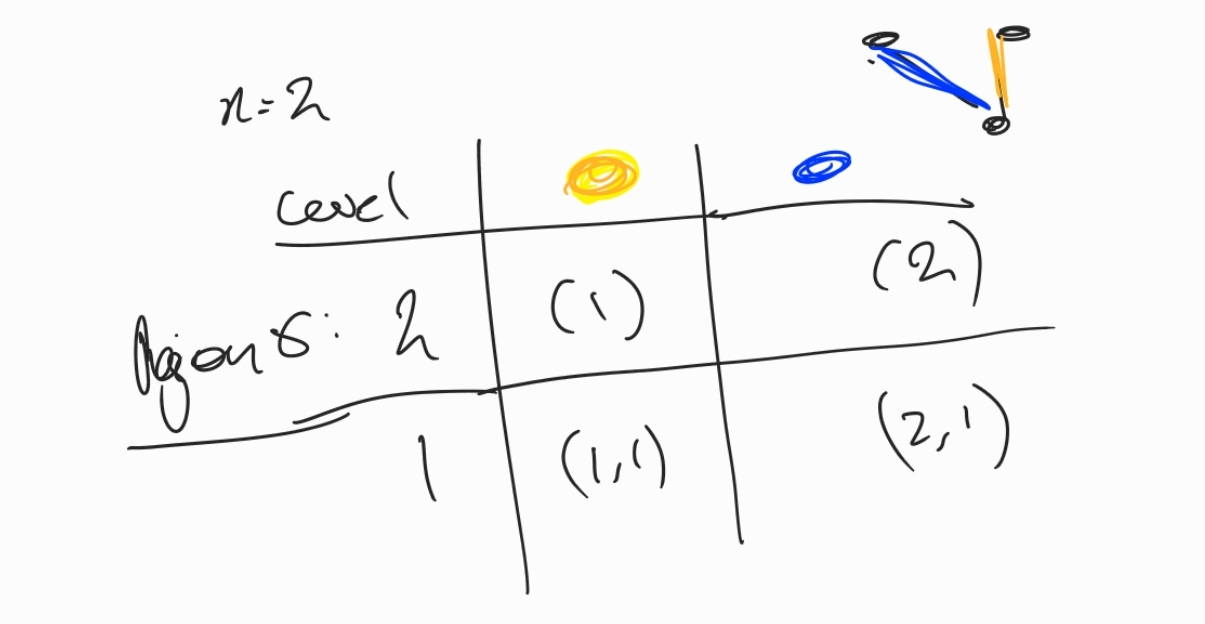
\includegraphics[scale=0.25,angle=0]{29072020 pics/n2bookkeeping.jpg}  
    \caption{}
    \label{}
\end{figure}

The table above shows vertically the regions which combine to give the higher dimensional region above, and horizontally the columns show the region number of $\mathbb{R}^n$.
        
        
        \end{example}
        
     \begin{example}
               For $n=3$ we have the following:
               
                            \begin{figure}[H]
    \centering
 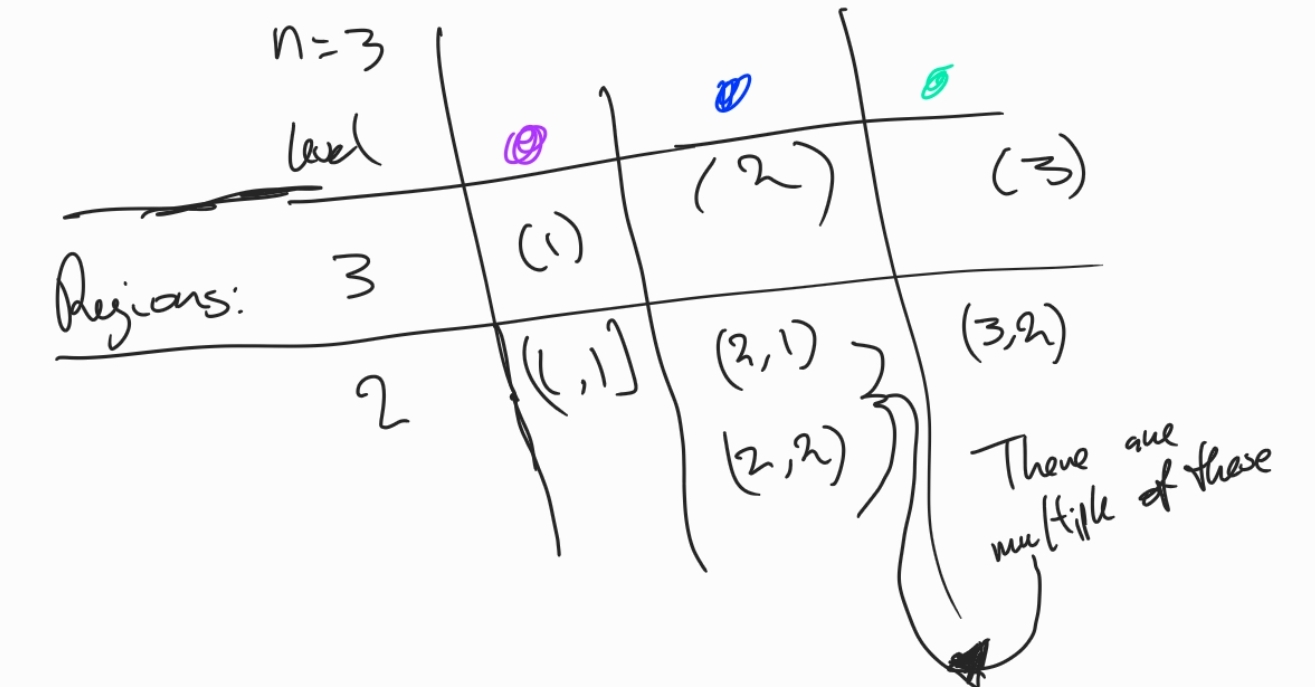
\includegraphics[scale=0.25,angle=0]{29072020 pics/n3bookkeeping.jpg}  
    \caption{}
    \label{}
\end{figure}
        \begin{figure}[H]
    \centering
 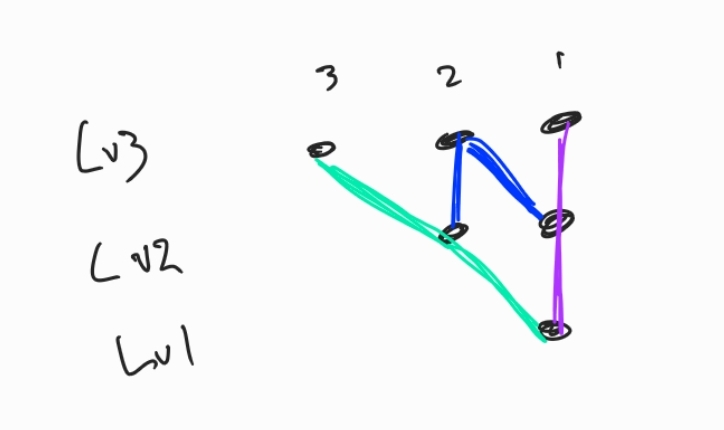
\includegraphics[scale=0.25,angle=0]{29072020 pics/n3bookdiagram.jpg}  
    \caption{}
    \label{}
\end{figure}

 For example the function with $(2,1)$ is from region $2$ of $\mathbb{R}^3$ and region $1$ of $\mathbb{R}^2$.

     \end{example}

\begin{example}
                  For $n=4$ we have the following:
                  
                          \begin{figure}[H]
    \centering
 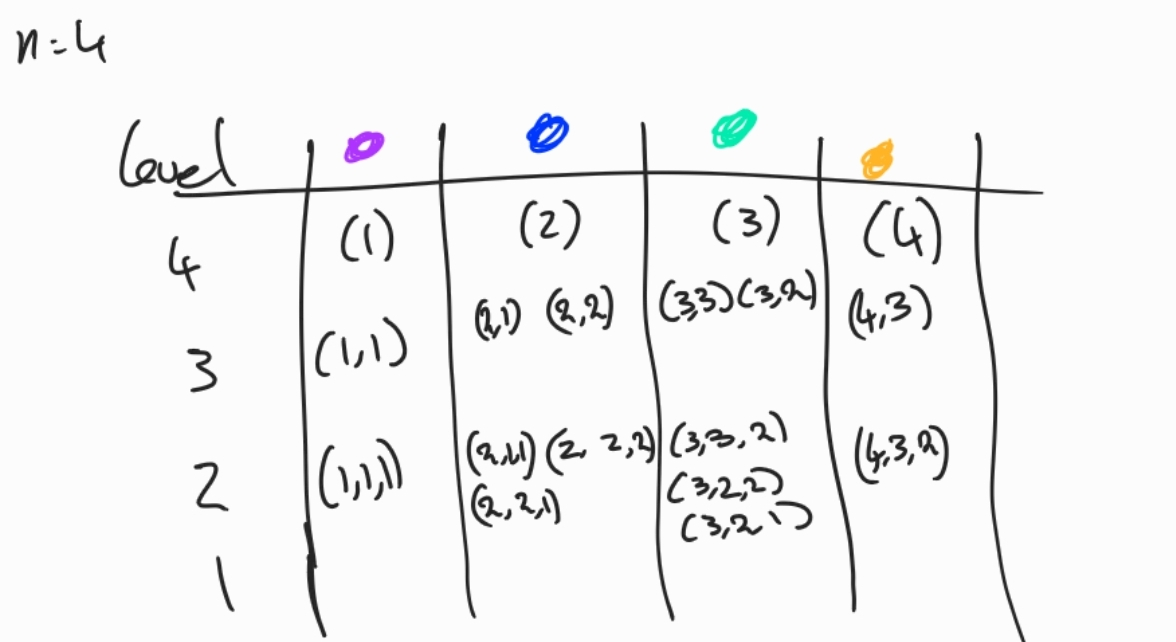
\includegraphics[scale=0.25,angle=0]{29072020 pics/n4bookkeeping.jpg}  
    \caption{}
    \label{}
\end{figure}
           \begin{figure}[H]
    \centering
 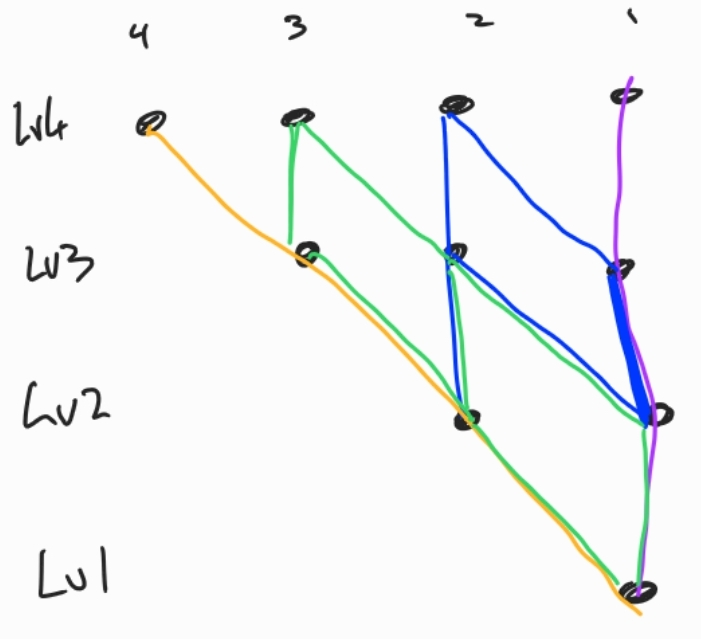
\includegraphics[scale=0.25,angle=0]{29072020 pics/n4bookdiagram.jpg}  
    \caption{}
    \label{}
\end{figure}
\end{example}
     
     
     \begin{titlemize}{Notes for $(m)$ diagram}
\item Q: In what way can we move in the diagram for $(m)$? only by 1 or 0 or by 2? Look at SA definition. They want to move to the right if they have the option. 
\end{titlemize}

\end{itemize}


\section{Theory}


 
  Define $\mathbb{Z}^{ 2^{[n]} \setminus \{\emptyset\} } := \{ f : 2^{[n]} \setminus \{\emptyset\} \rightarrow \mathbb{Z} \} $. 
    
    
Define $P_n ^{+} := 2^{[n]} \setminus \{\emptyset\}$ with $f: P_n ^{+}  \rightarrow \mathbb{Z}$ is mildly super additive.



The space of mildly super additive functions is given by $$\tilde{P_n}=\{ f: 2^{[n]} \setminus \{\emptyset\} \rightarrow \mathbb{Z} \mid SA\}.$$

The super-additive (SA) condition is given by letting $I,J \in  2^{[n]}$ with $I \cap J = \emptyset$, then 

\begin{equation}\label{SA}
 f(I \cup J)=
    \begin{cases}
     f(I) + f(J) \\
     f(I) + f(J) +1.\\
    \end{cases}       
\end{equation}

Where $ 2^{[n]}:=P(\{1,\dots,n\})$ is the the power set.  The SA condition is necessary condition for $R_f\ne \emptyset$.
\end{definition}

.

\begin{remark}
     $\tilde{P_n}$ parameterises all fine compactified universal $g=1$ Jacobians.
\end{remark}
    
    
\begin{definition}
The space of polytopes is denoted by $P_n$ and is the connected components of $\mathbb{R}^n \setminus  \cup H(S,k)$. 
\end{definition}

\begin{remark}
         Polytopes are the non-degenerating (wrt some stability conditions) parts connected components of $\mathbb{R}^n \setminus  \cup H(S,k)=: P_{1,n}$. The hyperplanes are locally finite and have no accumulation point, $\infin$ many translates.
\end{remark}

Polytopes can be obtained from function method by the following map, $\tilde{P_n} \rightarrow \{ \emptyset \} \cup P_{1,n}$ where $$f \mapsto R_{f}:=\{(x_1,\dots,x_n ) \subseteq \mathbb{R}^n\mid f(I) < \sum_{i\in I} x_i < f(I) +1 , \forall I \ne \emptyset \in 2^{[n]} \}.$$
    

        
        \begin{titlemize}{Practice with SA functions}
          \item  For $n=2$ we have $f(\{1\} \cup \{2\})= f(1)+f(2)=0+0=0$ or $f(\{1\} \cup \{2\})=f(1)+f(2)+1=1$.
            
            \item For $n=3$ note there is no choice in value for $f$ by condition (\ref{SA}) on $\{1,2,3\}$ as $\{1,2\}$ and $\{1,3\}$ have $\{1\}$ in common (see Example \ref{n=3}).
            
           \item For $n=4$ we have for the case where $f(I \cup J)=f(I) +f(J)$ the following possible values $$f(\{1,2\} \cup \{3,4\})= f(\{1,2\}) + f(\{3,4\}) =0+0 \text{ or } =0+1 \text{ or } =1+0 \text{ or }  1+1$$. In the case where  $f(I \cup J)=f(I) +f(J)+1$ we have  
             $$f(\{1,2\} \cup \{3,4\})= f(\{1,2\}) + f(\{3,4\}) +1= 0+0+1 \text{ or } \text{=other permutations} \text{ or }  =1+1+1.$$
             \item What values can max length (n) functions of a given take? They can take values $\{1,2,\dots, n-1\}$.
        \end{titlemize}
        

        
        \begin{example} {This is not true as $f$ does not have SA condition.}\\
        In $n=2$ case we get $R_f=\emptyset$ by setting
$f(\{ 1\}) = f( \{ 2\}) =0$ and $f(\{1,2\})=10$ then $R_f = \emptyset$. Then one has the following bounds  $0< f(1)=x_{1} <1 $ , $0< f(2) = x_{2} <1 $ and $10 < f(\{1,2\})=x_{1} +x_{2} <11$.

   \begin{figure}[H]
    \centering
 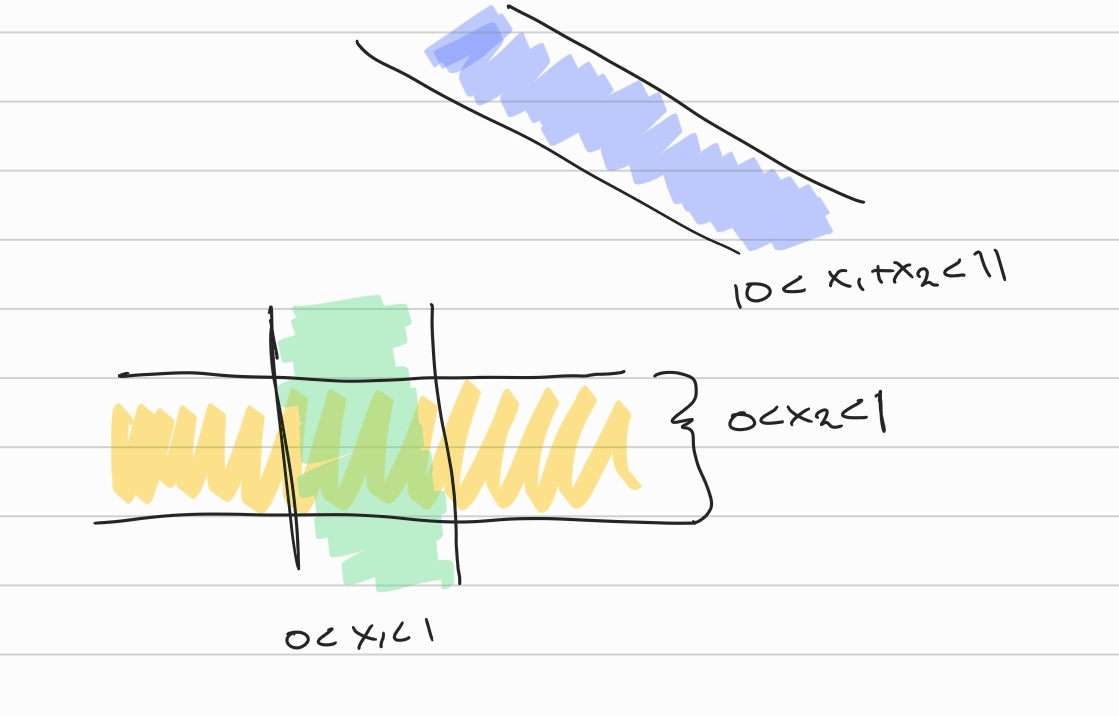
\includegraphics[scale=0.25,angle=0]{29072020 pics/n2emptyset.jpg}  
    \caption{}
    \label{off}
\end{figure}

        \end{example}
        


   
  For $f$ over $S$ one gets the interval of the polytopal hyperplane region $R_f$ which recaptures the hyperplanes conditions when the inequalities are equality this can however map to the empty set. Previously it was thought $\tilde{P_n} \leftrightarrow P_n$ but a counterexample exists. This is not the case.
    
    \begin{example}{Counterexample}\label{counter}       

    
      Consider $f \in \tilde{P_{5}}$ with $f(I)=0$ for $ I \nsupseteq \{ 1,3,5 \}$ or  $ I \nsupseteq \{ 2,4,5 \}$ and $f(\{I\}) = 1$ otherwise.
      
    \medskip 
    
             This is mildly super additive. We start by checking that the value $f(I)=1$ is allowed for $\{1,3,5\}$ and $\{2,4,5\}$, this is allowed by the condition $I \cap J = \emptyset$ for $\{1,3\}$ and $\{3,5\}$ as the intersection is non-empty and $\{1,3,5\}$ overlaps with $5$ with on $\{2,4,5\}$.
        
        \medskip
        We also see that $R_f=\emptyset$, as we have $1<x_1 + x_3 + x_5 <2$ and $0< x_2 +x_3 +x_5 <1$ and taking the difference gives $0<x_1 - x_2 <2$ which shows $x_1 > x_2$. Similarly take $0 < x_1 + x_4 + x_5 <1$ and $1 < x_2 +x_4 +x_5<2 $ and take the difference which gives $x_2 >x_1$ hence $R_f = \emptyset$ even if SA conditions holds. 
    \end{example}
    
        
    Let $c\in P_n$ and if $\underline {x} \in c$ then $$\kappa_S < \sum_{S} x_i < \kappa_S + 1.$$ With $c \mapsto \kappa_S$ ie. $\alpha(c)(S)=\kappa_S$. We claim $\alpha$ is injective. We aim to show the following.
    
     
    \begin{lemma}
    Let $n \le 4$ then $\alpha_n: {P_n}  \rightarrow \tilde{P_{n}}$ is a bijection. 
    \end{lemma}
 
 \begin{figure}[H]
    \centering
 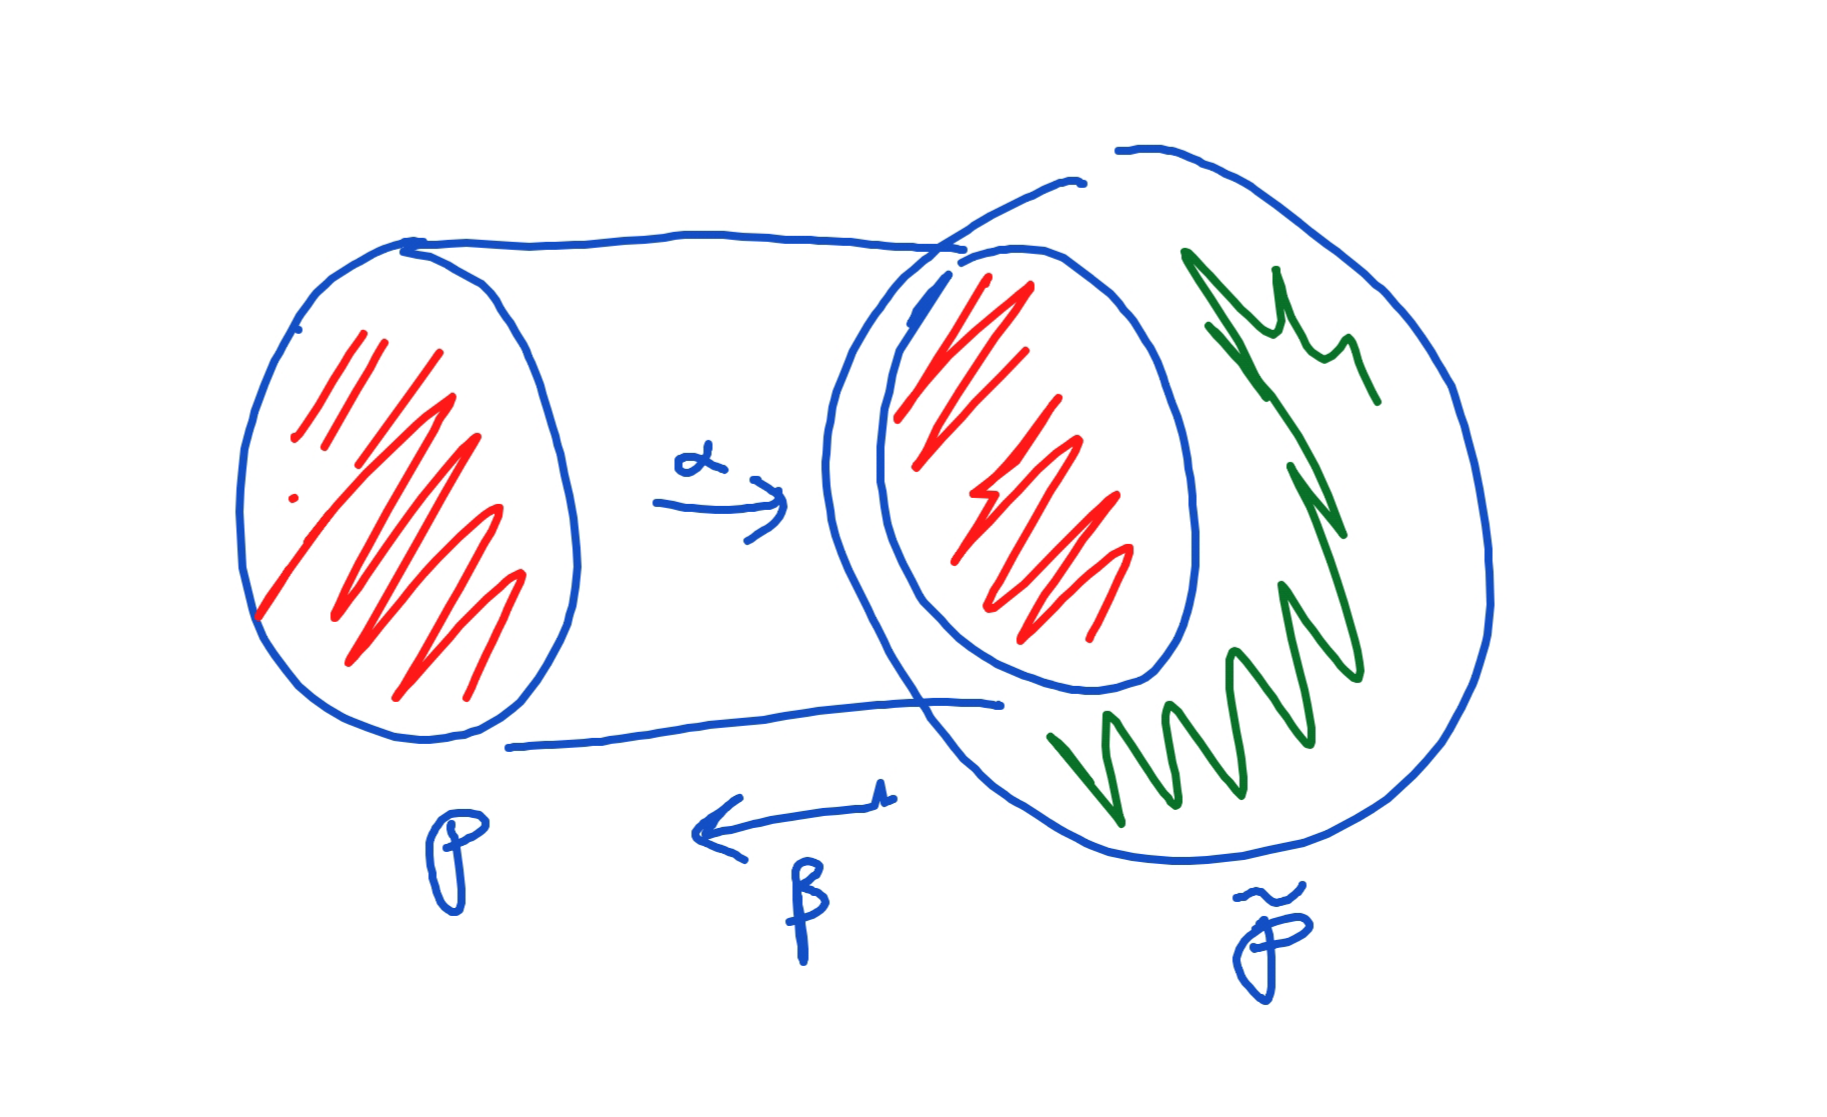
\includegraphics[scale=0.15,angle=0]{29072020 pics/alphabetamap.png}  
    \caption{}
    \label{}
\end{figure}
 
   Consider the opposite map $\beta: \tilde{P_{1,n}} \rightarrow P_n \cup \emptyset$ which is surjective. On the red part of the diagram, $\beta$ is the inverse of $\alpha$ and green is sent to the empty set (consider Example \ref{counter} there $\beta(f)=\emptyset$).
 
    \medskip 
    
    
    \begin{remark}
             The Polytope method is a sub-question of the Function Method
    \end{remark}
        Consider the following subsets: 
            $$P_n ^{'} = \{ c \in P_n \mid c \subseteq [0,1]^n\} \subseteq  P_n$$
            
            The hypercube is given by setting the function value for singletons to be $f(\{i\})=0$.

            
            $$\tilde{P_n}^{'} = \{ f \in  \tilde{P_{n}} \mid  f (\{ i \})=0 \quad \text{ s.t }  0 \le i\le n \} \subseteq \tilde{P_n}$$
            
            
    Restricting to $\alpha \mid_{P_n ^{'}} : P_n ^{'} \rightarrow \tilde{P_n}^{'}$ and  $\beta \mid _{\tilde{P_n}} : \tilde{P_n} \rightarrow P_{n}^{'} \cup \emptyset$. 
    
    \medskip
    
     There also exists a map $\mathbb{Z}^{ 2^{[n]} \setminus \emptyset} := \{ f : S \rightarrow  2^{[n]} \} \rightarrow  \emptyset \cup P_{1,n}$, wher $\tilde{P_n}   \subseteq \mathbb{Z}^{ 2^{[n]} }$.  The set $\mathbb{Z}^{ 2^{[n]} \setminus \emptyset}$ has no SA conditions and if $f \notin \tilde{P_n}  \implies R_f=\emptyset$.

\section{Obtaining hypercube count for $n=2,3,4$ by counting functions}

We now aim to determine the $n=2,3,4$ count for SA functions by studying the subsets $I,J$ in $ 2^{[n]}$ and then reduce to the hypercube count. For all functions in this section we require $f(\{i\})=0$

\begin{example}
For $n=2$ we have ${}^{1}f^{(1)}_{2}(\{1,2\})=0$ or ${}^{2}f^{(2)}_{2}(\{1,2\})=1$. 
      
       \begin{figure}[H]
    \centering
 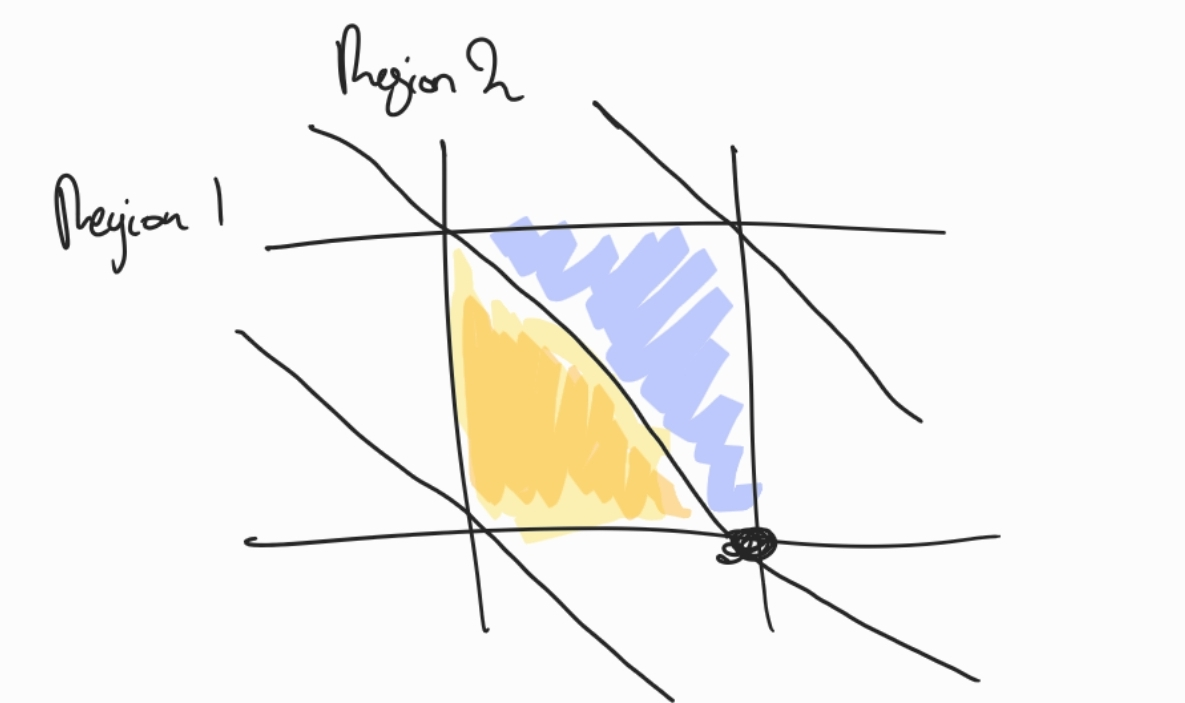
\includegraphics[scale=0.25,angle=0]{29072020 pics/n2regionsfunctionmeth.jpg}  
    \caption{}
    \label{}
\end{figure}

These are the only functions as otherwise consider Figure \ref{off}.



\end{example}

 To make counting arguments easier for larger $n$. For example we will split the $\mathbb{R}^3$ arrangement into regions as follows.

         \begin{figure}[H]
    \centering
 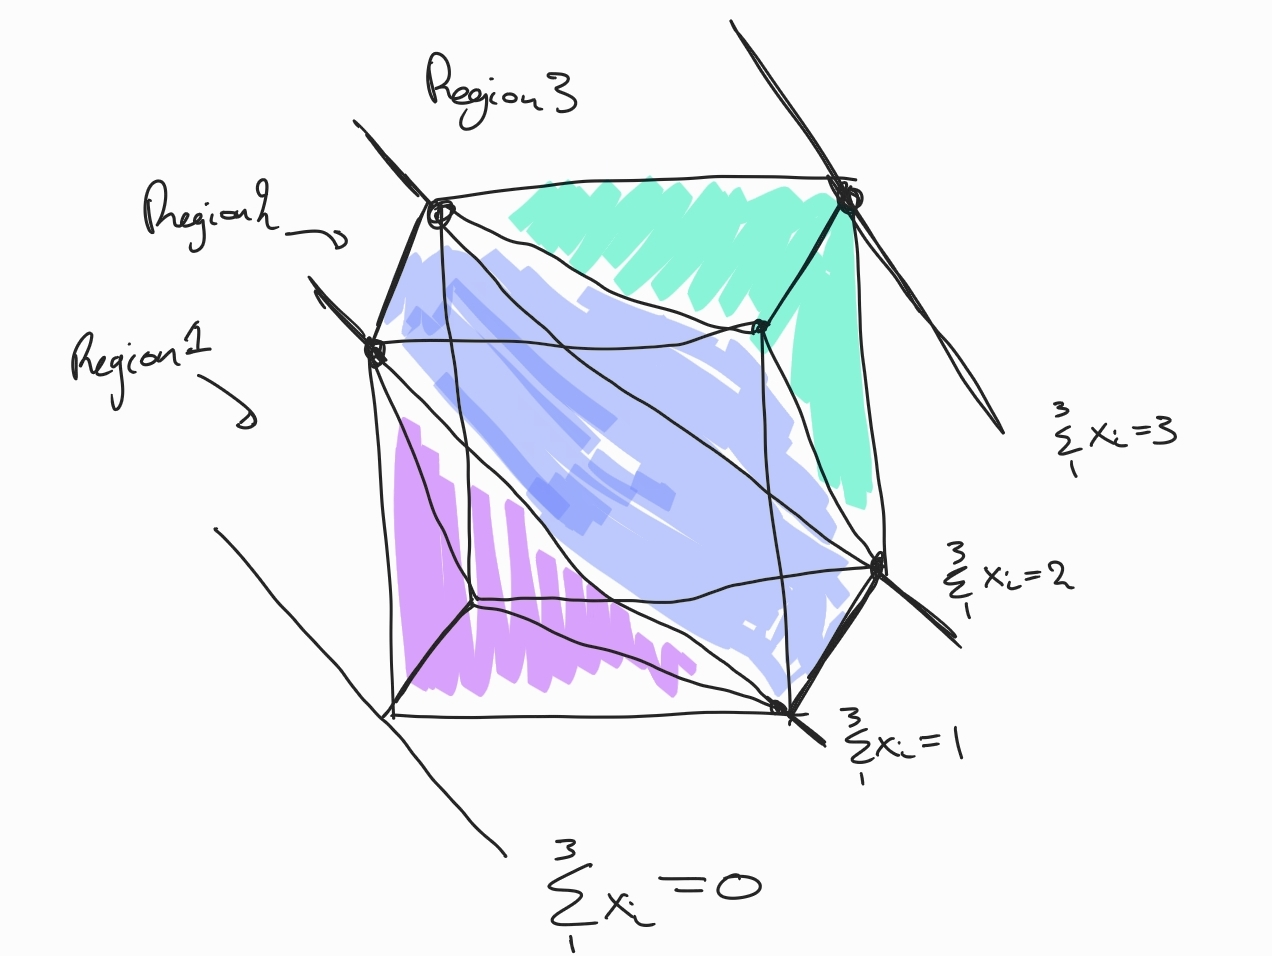
\includegraphics[scale=0.25,angle=0]{29072020 pics/n3functionMethodregions.jpg}  
    \caption{}
    \label{r3regions}
\end{figure}

\begin{definition}\label{region}
The region number is given by splitting the interval $[0,1]$ by the key intersection points (given by hyperplanes of length $m< n$) and hyperplanes of length $n$ where length is the number of $x_i$ terms in the defining equation. 
\end{definition}

\begin{example} The regions for $n=3$ are the following,
  \begin{figure}[H]
    \centering
 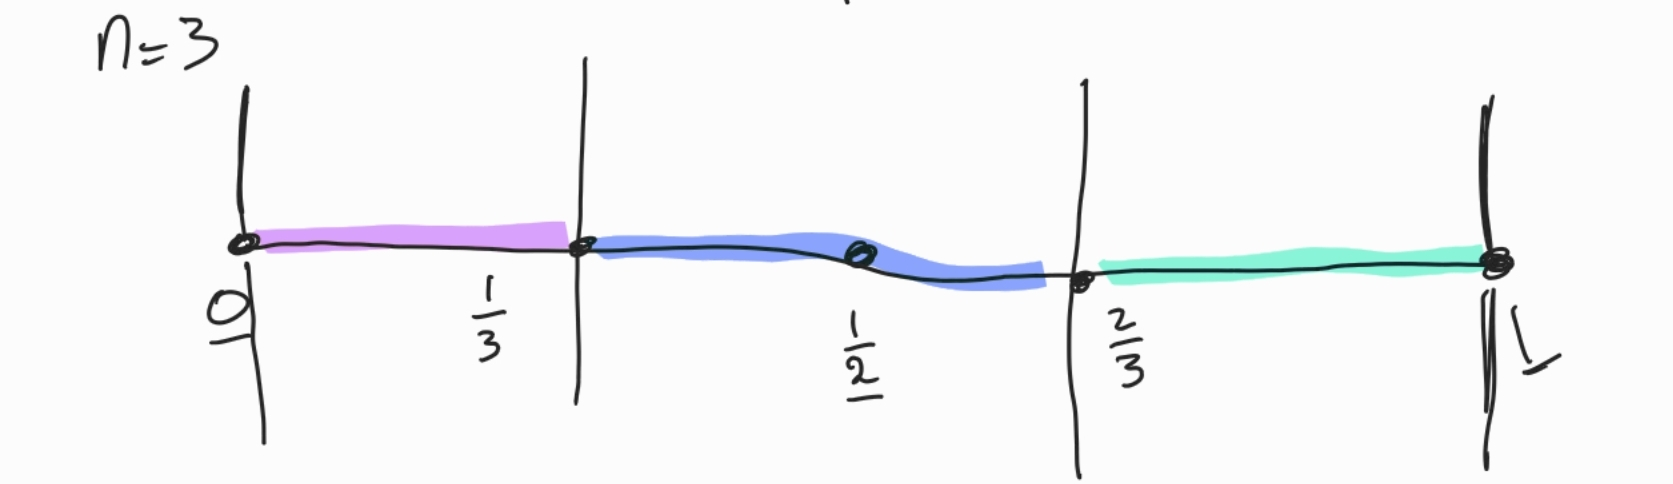
\includegraphics[scale=0.25,angle=0]{29072020 pics/n3regionsline.jpg}  
    \caption{Representation of Figure \ref{r3regions} regions}
    \label{r3regionsline}
\end{figure}

For $\mathbb{R}^n$ there are $n-1$ hyperplanes intersecting there line corresponding to $\frac{1}{n} \dots \ \frac{n-1}{n}$.

\begin{example}
Here is the regions of $n=7$

          
          \begin{figure}[H]
    \centering
 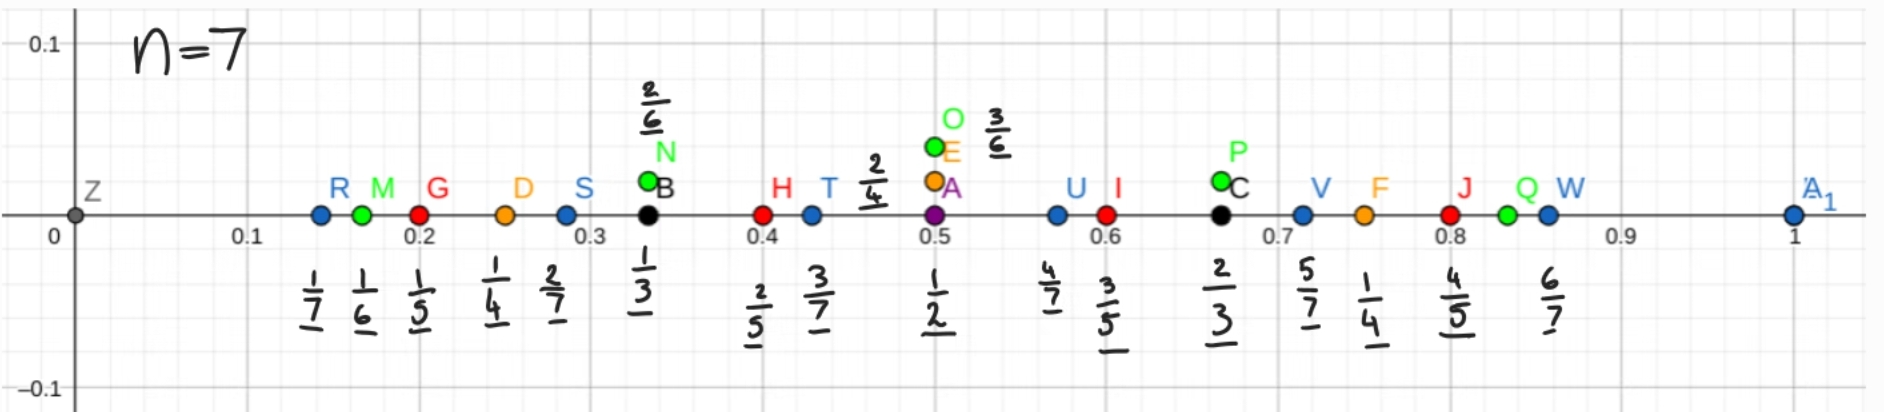
\includegraphics[scale=0.25,angle=0]{29072020 pics/n=7regions.jpg}  
    \caption{$n=7$ regions projected to a line}
    \label{}
\end{figure}
\end{example}



\begin{example} \label{n=3}
For $n=3$ we have  $2^{[3]}\setminus \emptyset= \{ \{1,2,3\}, \{1,2\},\{1,3\},\{2,3\},\{1\} ,\{2\} ,\{3\} \} $. On $\{1,2,3\}$ its value is either $0,1,2$ for region $1,2,3$ respectively. On $2$-tuples there is a choice in value by disjointedness of $\{1\}$ and $\{2\}$,

\begin{equation}
 f(\{1,2\})=
    \begin{cases}
     f(\{1\}) + f(\{2\}) \\
     f(\{1\}) + f(\{2\}) +1\\
    \end{cases}       
\end{equation}

First we give the function corresponding to the corner closest to $\underline{0}$ (called region $1$). Function values where determined starting with the value on $\{1,2,3\}$.


\begin{center}
   \begin{tabular}{|c||c||c|c|c|}
   \hline
X&${}^{1}f^{(1)}_{3}(\{1,2,3\})=0$ 
&${}^{1}f^{(1,1)}_{2}(\{1,2\})=0$
&${}^{1}f^{(1,1)}_{2}(\{1,3\})=0$ 
&${}^{1}f^{(1,1)}_{2}(\{2,3\})=0$\\
\hline
\end{tabular} 
\end{center}

Note given $x_1+ x_2 +x_3=0$ we cannot have $x_1+x_2>0$ otherwise $x_3<0$ which contradicts our assumption of $f(\{x_i\})=0$. Next we give the function corresponding to region $3$ which is given by,
\begin{center}
 \begin{tabular}{|c||c||c|c|c|}
 \hline
Y&${}^{2}f^{(3)}_{3}(\{1,2,3\})=2$
&${}^{2}f^{(3,2)}_{2}(\{1,2\})=1$
&${}^{2}f^{(3,2)}_{2}(\{1,3\})=1$
&${}^{2}f^{(3,2)}_{2}(\{2,3\})=1$.\\
\hline
\end{tabular}   
\end{center}

This is the only function allowed as otherwise contradicts our assumption of $f(\{x_i\})=0$. We now we examine region 2. 

\begin{center}
\begin{tabular}{ |c||c||c|c|c| } 
  \hline
A&${}^{3}f^{(2)}_{3}(\{1,2,3\})=1$&
${}^{3}f^{(2,1)}_{2}(\{1,2\})=0$&
${}^{3}f^{(2,1)}_{2}(\{1,3\})=0$&
${}^{3}f^{(2,1)}_{2}(\{2,3\})=0$\\
 \hline
 \hline
B_1 &${}^{4}f^{(2)}_{3}(\{1,2,3\})=1$&
${}^{4}f^{(2,1)}_{2}(\{1,2\})=0$ &
${}^{4}f^{(2,1)}_{2}(\{1,3\})=0$ &
${}^{4}f^{(2,2)}_{2}(\{2,3\})=1$ \\
 \hline
B&${}^{5}f^{(2)}_{3}(\{1,2,3\})=1$&
${}^{5}f^{(2,1)}_{2}(\{1,2\})=0$&
${}^{5}f^{(2,2)}_{2}(\{1,3\})=1$&
${}^{5}f^{(2,1)}_{2}(\{2,3\})=0$\\
 \hline
B&${}^{6}f^{(2)}_{3}(\{1,2,3\})=1$&
${}^{6}f^{(2,2)}_{2}(\{1,2\})=1$&
${}^{6}f^{(2,1)}_{2}(\{1,3\})=0$&
${}^{6}f^{(2,1)}_{2}(\{2,3\})=0$\\
 \hline
 \hline
C&${}^{7}f^{(2)}_{3}(\{1,2,3\})=1$&
${}^{7}f^{(2,2)}_{2}(\{1,2\})=1$&
${}^{7}f^{(2,2)}_{2}(\{1,3\})=1$&
${}^{7}f^{(2,1)}_{2}(\{2,3\})=0$\\
 \hline
C&${}^{8}f^{(2)}_{3}(\{1,2,3\})=1$&
${}^{8}f^{(2,2)}_{2}(\{1,2\})=1$&
${}^{8}f^{(2,1)}_{2}(\{1,3\})=0$&
${}^{8}f^{(2,2)}_{2}(\{2,3\})=1$\\
 \hline
C&${}^{9}f^{(2)}_{3}(\{1,2,3\})=1$&
${}^{9}f^{(2,1)}_{2}(\{1,2\})=0$&
${}^{9}f^{(2,2)}_{2}(\{1,3\})=1$&
${}^{9}f^{(2,2)}_{2}(\{2,3\})=1$\\
 \hline
 \hline
D&${}^{10}f^{(2)}_{3}(\{1,2,3\})=1$& 
${}^{10}f^{(2,2)}_{2}(\{1,2\})=1$&
${}^{10}f^{(2,2)}_{2}(\{1,3\})=1$&
${}^{10}f^{(2,2)}_{2}(\{2,3\})=1$\\
 \hline
\end{tabular}
\end{center}

There are $ 3 \choose 0$ many $A$'s, $ 3 \choose 1$ many $B$'s, $ 3 \choose 2$ many $C$'s and $ 3 \choose 3$ many $D$'s (ways to assign the value 1 to ${}^{i}f^{(m)}_{2}(\{r,s\})$). 
\begin{remark}
     From this data we can given function give a specific polytope of the cube.    
\end{remark}

Therefore we have $10$ functions in total.


\end{example}

\begin{example}\label{n=4}
For $n=4$ we have the following power set,
\begin{align*}
    2^{[4]} \setminus \emptyset&= \{\{1,2,3,4\},\{1,2,3\},\{1,2,4\},\{1,3,4\},\{2,3,4\},\\
    &\{1,2\},\{1,3\},\{1,4\},\{2,3\},\{2,4\},\{3,4\},\{1\},\{2\},\{3\},\{4\}\}
\end{align*}

The regions are also described by the following.


      \begin{figure}[H]
    \centering
 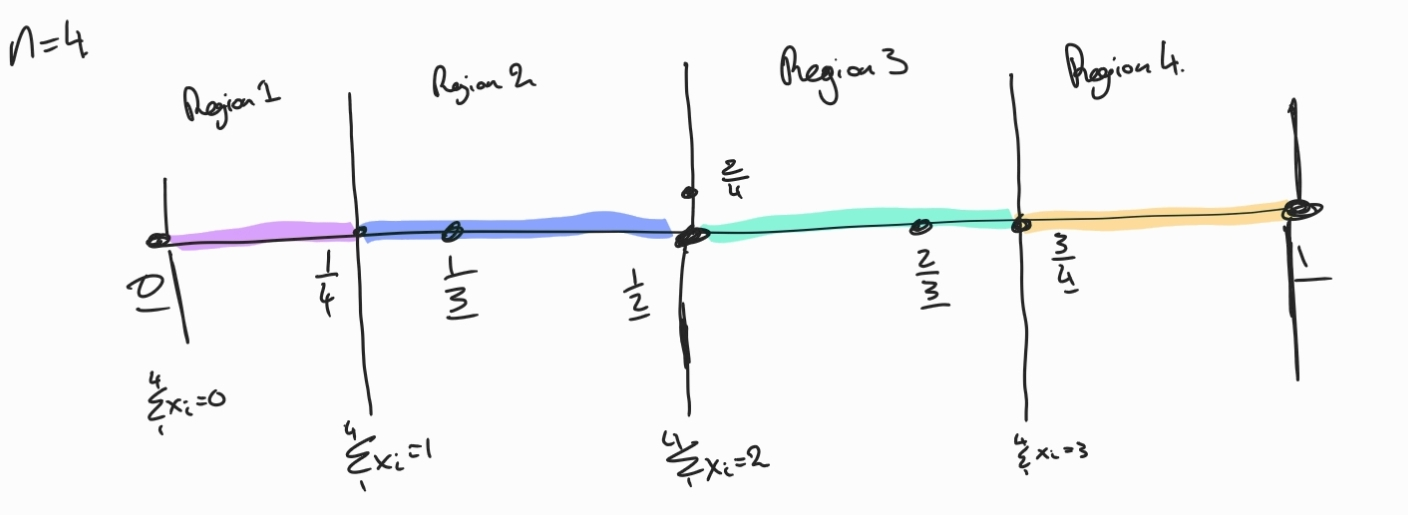
\includegraphics[scale=0.25,angle=0]{29072020 pics/n4regionsline.jpg}  
    \caption{}
    \label{}
\end{figure}

The possibilities for level $3$ values are $4 \choose 0$ of type $(0,0,0,0)$, $4 \choose 1$ of type $( 1,0,0,0)$,  $4 \choose 3$ of type $(1,1,0,0)$ and  $4 \choose 4$ of type $(1,1,1,1)$. For the region $1$ we have,

\begin{center}
   \begin{tabular}{|c||c||c|c|c|c|}
   \hline
$\alpha$ &${}^{1}f^{(1)}_{4} (\{1,2,3,4\})=0$ & & &  \\
\hline
 &${}^{1}f^{(1,1)}_{3} (\{1,2,3\})=0$ &${}^{1}f^{(1,1)}_{3} (\{1,2,4\})=0$ &${}^{1}f^{(1,1)}_{3} (\{1,3,4\})=0$ &${}^{1}f^{(1,1)}_{3} (\{2,3,4\})=0$ \\
\hline
\end{tabular} 
\end{center}

By $X$ of Example $\ref{n=3}$ the functions values are of the form ${}^{1}f^{(1,1,i)}_{2}(\{r,s\})=0$ for $1 \le r,s \le 4$ where $(m)=(1,1)$ denotes region $1$ of $\mathbb{R}^4$ and region $1$ of $\mathbb{R}^3$ and the $i$ term will be $1$ as the value is $0$. By symmetry we have a similar circumstance at region $4$. For the $4$th region we have following,

\begin{center}
   \begin{tabular}{|c||c||c|c|c|c|}
   \hline
$\omega$ &${}^{p}f^{(4)}_{4} (\{1,2,3,4\})=3$ & & &  \\
\hline
 &${}^{p}f^{(4,3)}_{3} (\{1,2,3\})=2$ &${}^{p}f^{(4,3)}_{3} (\{1,2,4\})=2$ &${}^{p}f^{(4,3)}_{3} (\{1,3,4\})=2$ &${}^{p}f^{(4,3)}_{3} (\{2,3,4\})=2$ \\
\hline
\end{tabular} 
\end{center}

 where we will use the place holder $p$ for the number of the equation. By $Y$ all level $2$ functions values are of the form ${}^{p}f^{(4,3,i)}_{2}(\{r,s\})=1$ for $1 \le r,s \le 4$ and the $i$ term will be $2$ as the value is $1$. Hence the at level $2$ function value is of the form ${}^{p}f^{(4,3,2)}_{2}(\{r,s\})=1$.\\



By symmetry it should be enough to check region $2$ then we are done. As there are choices to be made at level $2$ as seen in the $n=3$ case, we will hold off assigning the function a number until we have given a value for the level $2$ terms. We will follow this procedure when counting functions.

\begin{titlemize}{Procedure for counting functions in $n=4$}
   \item Group functions by region. 

\item Move to level 3 values, counting the different combination by type e.g $(1,1,0,0)$ and their permutations.

\item Fix a combination type e.g $(0,1,1,0)$. The same function applies to all $I \in 2^{[4]}$ in particular the $4 \choose 2$ many $2$-tuples. 


\item Move to level $2$ values and determine the number of functions similar to $n=3$ but be careful as the $0$'s in level $3$ combination (0,1,1,0) force level $2$ values.
\end{titlemize}



We start with the following,

\begin{center}
   \begin{tabular}{|c||c||c|c|c|c|}
   \hline
$\beta$ &${}^{i}f^{(2)}_{4} (\{1,2,3,4\})=1$ & & &  \\
\hline
 &${}^{i}f^{(2,2)}_{3} (\{1,2,3\})=1$ &${}^{i}f^{(2,1)}_{3} (\{1,2,4\})=0$ &${}^{i}f^{(2,1)}_{3} (\{1,3,4\})=0$ &${}^{i}f^{(2,1)}_{3} (\{2,3,4\})=0$ \\
\hline
\end{tabular} 
\end{center}

As ${}^{i}f^{(2,2)}_{3} (\{1,2,3\})=1$ there are choices to be made at level $2$. For the sake of notation we will write the terms but leave out the value as they are yet to be assigned,

\begin{align*}
    {}^{i}f^{(2,2,-)}_{2} (\{1,2\})&=-,\\ {}^{i}f^{(2,2,-)}_{2} (\{1,3\})&=-,\\ {}^{i}f^{(2,2,-)}_{2} (\{2,3\})&=-.
\end{align*}

 There are $8$ choices here which we made in the $n=3$ case. There are $ 4 \choose 1$ permutations of $(1,0,0,0)$ at level $3$. This gives $4*8=32$ functions.

Now we consider the level $3$ set the values as of type $(1,1,0,0)$ there are $4 \choose 2$ permutations. 

\begin{center}
   \begin{tabular}{|c||c||c|c|c|c|}
   \hline
$\gamma$ &${}^{i}f^{(2)}_{4} (\{1,2,3,4\})=1$ & & &  \\
\hline
 &${}^{i}f^{(2,2)}_{3} (\{1,2,3\})=1$ &${}^{i}f^{(2,1)}_{3} (\{1,2,4\})=1$ &${}^{i}f^{(2,1)}_{3} (\{1,3,4\})=0$ &${}^{i}f^{(2,1)}_{3} (\{2,3,4\})=0$ \\
\hline
\end{tabular} 
\end{center}

Naively we try for each ${}^{i}f^{(2,2)}_{3} (I)=1$ we get $8$ possibilities of level $2$ functions values. Hence for $\gamma$ there are $4 \choose 2$ choices giving $16 * 6=96$. 

\begin{remark}
     We need to consider the overlap of values at lower levels. Consider (\ref{SA}) in regards to $\{1,2,3,4\}$ and the disjointedness of $\{1,2\}$ and $\{3,4\}$. 
\end{remark}

There is overlap of level $2$ functions value for ${}^{i}f^{(2,2)}_{3} (I)=1$ (see Figure \ref{overlap}). 


      \begin{figure}[H]
    \centering
 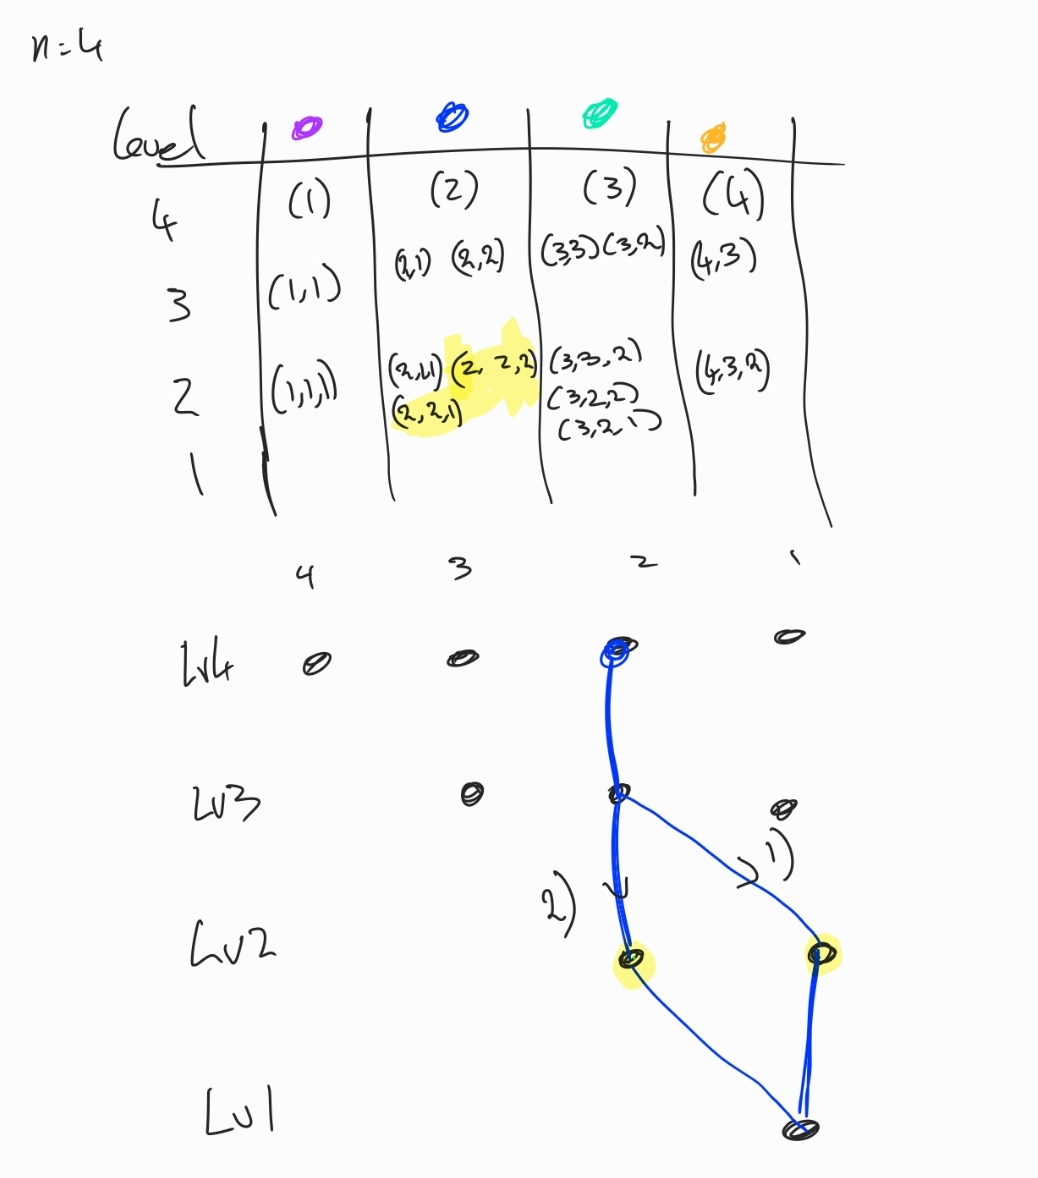
\includegraphics[scale=0.25,angle=0]{29072020 pics/n4bookkeepingcalc.jpg}  
    \caption{}
    \label{overlap}
\end{figure}

 I want to compare the level two terms for ${}^{i}f^{(2,2)}_{3} (\{1,2,3\})=1$ and ${}^{i}f^{(2,2)}_{3} (\{1,2,4\})=1$. These give the same terms as seen in the $n=3$ case but the $3$ and $4$ are switched. Proceed not naively starting with level $3$ with value $0$ of $\gamma$.\\

As ${}^{i}f^{(2,1)}_{3} (\{1,3,4\})=0$ and ${}^{i}f^{(2,1)}_{3} (\{2,3,4\})=0$ we have 
$$^{i}f_{2}(I)=0  \text{ for } I=\{ \{1,3\}, \{3,4\},\{1,4\},\{2,3\},\{3,4\},\{2,4\} \}.$$

When determining the values for 2-tuples from ${}^{i}f^{(2,2)}_{3} (\{1,2,3\})=1$ and ${}^{i}f^{(2,2)}_{3} (\{1,2,4\})=1$ this forces the value for $$I=\{ \{1,3\},\{1,4\},\{2,3\},\{2,4\} \}$$ to be $0$ with $\{1,2\}$ free to be either $0$ or $1$. The term $\{3,4\}$ is also free to be $0$ or $1$. Hence there are $6*2$ choices here.


\begin{remark}   
The values on the levels below $n$ are determined by the value at level $n$. If the value at level $(m)$ is $0$ then the value for all levels below that is also $0$. (Check/Wishful thinking?)(Rigorise use of $(m)$ diagram).
\end{remark}

\begin{titlemize}{Using diagram for $(m)$}
\item Consider $\gamma$ for a fixed function $k$ such that  ${}^{k}f^{(2,1)}_{3} (\{1,3,4\})=0$ and ${}^{k}f^{(2,2)}_{3} (\{1,2,3\})=1$, we aim to determine the value of ${}^{k}f^{(2,1,-)}_{2} (\{1,3\})=-$  and ${}^{k}f^{(2,2,-)}_{2} (\{1,3\})=-$. First we have ${}^{k}f^{(2,1,1)}_{2} (\{1,3\})=0$ by ${}^{k}f^{(2,1)}_{3} (\{1,3,4\})=0$. For the latter one has either ${}^{k}f^{(2,2,2)}_{2} (\{1,3\})=1$ or ${}^{k}f^{(2,2,1)}_{2} (\{1,3\})=0$ see Figure \ref{overlap}. 
   
\end{titlemize}



We now move onto the last case, consider

\begin{center}
   \begin{tabular}{|c||c||c|c|c|c|}
   \hline
$\delta$ &${}^{i}f^{(2)}_{4} (\{1,2,3,4\})=1$ & & &  \\
\hline
 &${}^{i}f^{(2,2)}_{3} (\{1,2,3\})=1$ &${}^{i}f^{(2,2)}_{3} (\{1,2,4\})=1$ &${}^{i}f^{(2,1)}_{3} (\{1,3,4\})=1$ &${}^{i}f^{(2,1)}_{3} (\{2,3,4\})=0$ \\
\hline
\end{tabular} 
\end{center}

As ${}^{i}f^{(2,1)}_{3} (\{2,3,4\})=0$ we have 
$$^{i}f_{2}(J)=0  \text{ for } J=\{\{2,4\},\{3,4\},\{2,3\}\}.$$

and for subests $\{\{1,2\},\{1,3\},\{1,4\}\}$ we have $^{i}f_{2}(J)=0,1$. Hence giving a total of $2^3=8$ combinations. 




In conclusion we have the total given as follows. From $\beta$ for level $3$ choice of type $(1,0,0,0)$ we have have ${4 \choose 1} * 8=32$. From $\gamma$ for level $3$ choice of type $(1,1,0,0$) type we have ${4 \choose 2} * 2 =12$. From $\delta$ for level $3$ choice of type $(1,1,1,0$) type we have${4 \choose 3} * 8=32$. For each corner $\alpha$ of type $(0,0,0,0)$ and $\omega$ of type $(1,1,1,1)$ we get $2$. In total we have $1+76+76+1=154$.

\printindex

\bibliographystyle{alpha}
\bibliography{bibtex}



\end{document}


